\documentclass{article}
 \usepackage{times,alltt,xspace}
 \usepackage{epsfig,subfig,graphicx}
 \usepackage{algorithm}
 \usepackage{algpseudocode}
 \usepackage{amsmath,amsfonts,amstext,amssymb,textcomp}
 \usepackage{multicol}
 %\usepackage{enumitem}
 \usepackage{url}
 \newtheorem{lemma}{Lemma}
 \newtheorem{theorem}{Theorem}
 \newtheorem{conjecture}{Conjecture}
 \newtheorem{corollary}{Corollary}
 \newtheorem{proof}{Proof}
 \usepackage{setspace}
 \usepackage{txfonts}
 \usepackage{xcolor,colortbl}
 \usepackage{booktabs}
 \usepackage{tikz}
 \usepackage[]{caption, subfig}

\begin{document}

\section{Query Optimizer Integration} \label{integration}

In the earlier sections, given a user query, the modified operator
implementations were used for the \emph{standard} plan choice of the PostgreSQL
optimizer. That is, while the execution engine was PCM-conscious, the presence
of PCM was completely \emph{opaque} to the optimizer.  However, given the
read-write asymmetry of PCM in terms of both latency and wear factor, it is
possible that alternative plans, capable of providing better performance
profiles, may exist in the plan search space. To discover such plans, the
database query optimizer needs to incorporate PCM awareness in both the
operator cost models and the plan enumeration algorithms.

Current query optimizers typically choose plans using a latency-based costing
mechanism. We revise these models to account for the additional latency
incurred during writes. Additionally, we introduce a new metric of \emph{write
cost} in the operator cost model, representing the incurred writes for a plan
in the PCM environment, using the estimators described in Sections~\ref{sort}
to \ref{gby}.  We henceforth refer to the latency cost and the write cost of a
plan as {\bf LC} and {\bf WC}, respectively.

A new user-defined parameter, called the \emph{latency slack}, is incorporated
in the query optimizer.  This slack, denoted by $\lambda$, represents the
maximum relative slowdown, compared to the LC-optimal query plan, that is
acceptable to the user in lieu of getting better write performance.
Specifically, if the LC of the LC-optimal execution plan $P_o$ is $C_o$ and the
LC of an alternate plan $P_i$ is $C_i$, the user is willing to accept $P_i$ as
the final execution plan if $C_i \le (1+\lambda) C_o$. The $P_i$ with the least
WC satisfying this equation is considered the WC-optimal plan.

With the new metric in place, we need to revise the plan enumeration process
during the planning phase. This is because the native optimizer propagates only
the LC-optimal (and interesting order) plans through the internal nodes of the
dynamic programming lattice, which may lead to pruning of potential WC-optimal
plans. On the other hand, propagating the \emph{entire} list of sub-plans at
each internal node can end up in an exponential blow-up of the search space.  

We examined the nature of WC-optimal plans--by picking them out after
exhaustively enumerating all possible plans--for queries in the TPC-H
benchmark.  In all the experiments, we observed that the WC-optimal plan
invariably had the same \emph{join order} as the LC-optimal plan, albeit with
different operator algorithms. 
%An intuitive explanation of this observation is that join order chosen in the
%LC-optimal plan was picked up because it involved lesser data processing.
%Using a different join order then would translate to more data and
%consequently more writes.

%As an intermediate option between these two extremes, we use a heuristic
%propagation mechanism at each internal node, employing an algorithmic
%parameter, \emph{local threshold} $\lambda_l$ ($\ge\lambda$). Specifically,
%let $p_i$ and $p_o$ be a generic sub-plan and the LC-optimal sub-plan at a
%node, respectively, with $c_i$ and $c_o$ being their corresponding LC values.
%Now, along with the LC-optimal and interesting order sub-plans, we also
%propagate $p_i$ with the \emph{least} WC that satisfies $c_i \le (1+\lambda_l)
%c_o$. We observed that setting $\lambda_l = \lambda$ delivered reasonably good
%results in this respect.


%With the new metric in place, we need to revise the plan enumeration process
%during the planning phase. This is because the native optimizer propagates
%just the LC-optimal (and interesting order plans) through the internal nodes
%of the dynamic programming lattice, which may lead to pruning of potential
%WC-optimal plans. On the other hand, propagating the \emph{entire} list of
%sub-plans at each internal node can end up in an exponential blow-up of the
%search space. One immediate pruning technique is to to discard each plan that
%is dominated by some other plans in both LC and WC metrics.

Using this observation, the problem of finding the WC-optimal plan can be
mapped to the well known variation of the Knapsack Problem called the
\emph{Linear Multiple Choice Knapsack Problem (LMCKP)}. Each item in LMCKP has
a weight and a profit associated with it, and these items are divided into
disjoint sets. The objective is to pick up one item from each set in such a
manner that the total weight of the items is within the maximum weight allowed
in the knapsack, while maximising the total profit obtained. Formally stated,
the LMCKP problem is as follows \cite{lmckp}:

Given multiple sets $S_1, S_2,..., S_k$ of items to be packed in a
knapsack of capacity $c$. For each item $j \in S_i$ , there is an associated
profit $p_{ij}$ and a weight $w_{ij}$. The objective is to choose one item from
each class so as to maximize the profit sum while having the weight sum to be
within c. The Linear Multiple Choice Knapsack Problem (LMCKP) is  
thus formulated as:

maximize $z = \sum\limits_{i=1}^{k} \sum\limits_{j \in S_i}p_{ij} x_{ij}$

subject to $\sum\limits_{i=1}^{k} \sum\limits_{j \in S_i}w_{ij}  x_{ij} \le c$,

$\sum\limits_{j \in S_i}$    $ x_{ij} = 1, i = 1,...,k$

$0 \le x_{ij} \le 1$, $i = 1,...,k, j \in S_i$

All coefficients $p_{ij}, w_{ij}$, and $c$ are positive integers, and the
classes $S_1$,...$S_k$ are mutually disjoint, class $S_i$ having size $s_i$.
The total number of items is $n = \sum\limits_{i=1}^{k} n_i$

In our case, the sets $S_i$ correspond to the operators in the plan tree of a
query, with the items in a set mapping to the algorithms for an operator.  The
weight $w_{ij}$ of an item can be equated to the LC associated with an
algorithm. The profit $p_{ij}$ can similarly be mapped to a modified write cost
(MWC), obtained by subtracting the expected WC for each operator algorithm from
a common large positive constant.  Thus, given an LC limit $(1+\lambda)C_o$
(corresponding to knapsack capacity c), the LMCKP is equivalent to   the
problem of miniming WC (by maximising MWC) while having the total sum of each
operator's LC  to be within the LC limit.

With the above background in place, we describe our final algorithm which uses
two-passes to come up with the WC-optimal plan:

\subsection*{First Pass} In the first pass, we keep track of the LC-optimal and
an additional least WC plan (similar in the way of tracking interesting order
plans) at each node, using the usual dynamic programming procedure. If they
both are the \emph{same}, we skip the second pass and output that plan as the
solution. Otherwise, the LC-optimal cost $C_o$ is used as an input to the
second pass.

\subsection*{Second Pass} The second pass uses the $C_o$ obtained in the first
pass to derive the LC bound of $(1+\lambda)C_o$.  We use a greedy algorithm to
solve the LMCKP \cite{lmckp} which gives an optimal solution to the problem.  
The pseudo-code of this algorithm is outlined in Algorithm~\ref{alg:lmckp}. 

%\input{src/lmckp_algo}
\input{lmckp_algo}

There is a possibility that, for exactly one of the operators, the optimal
solution contains a weighted combination of two algorithms.  In that case, we
perform a partial execution of that operator with one algorithm and the
remaining execution with the second algorithm; the extent of each of those
executions being governed by their respective weights in the optimal solution.
For instance, in case of join nodes, we can divide the inner relation into two
parts in the ratio of the weights obtained from the greedy algorithm.  The
outer relation is joined with one inner relation part using the first
algorithm, and with the other part using the second algorithm.


\begin{figure}[htpb] \centering
	
\subfloat[Performance of Alternative Plans]{
%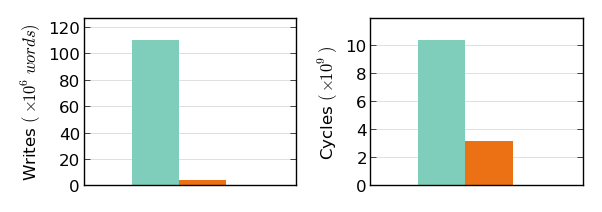
\includegraphics[height=29mm]{./fig/q13_alternate_plan.png} 
}

\subfloat[Overall performance comparison]{ \begin{small}

  %\begin{tabular}{p{3cm}p{2cm}p{2cm}p{2cm}p{2cm}}
  \begin{tabular}{p{3.5cm}c c c c} \toprule                                                                                                
  
  \textbf{Metric} & \textbf{Opt(PCM-O)} & \textbf{Opt(PCM-O) } &
\textbf{Opt(PCM-C)} & \textbf{Opt(PCM-C)}\\ & \textbf{Exec(PCM-O) } &
\textbf{Exec(PCM-C)} & \textbf{Exec(PCM-C)} & \textbf{Exec(PCM-O)}\\ \midrule                                                                                                
  
  \textbf{Mega Word-Writes} &  $233.6$ & $110.6$ & $4.66$ & $12.8$\\
\textbf{Giga Cycles} &  $13.1$ & $10.4$ & $3.2$ & $4.5$\\ \bottomrule
\end{tabular} \end{small} } \caption{Integration with Query Optimization and
Processing Engine} \label{fig:perf_comp} \end{figure}

In light of these modifications, let us revisit Query Q13, for which the
default plan was shown in Figure~\ref{fig:plan_trees}(a). With just the revised
latency costs (i.e. $\lambda$ = 0), the optimizer identified a new execution
plan wherein the merge left-join between the \textit{customer} and
\textit{orders} tables is replaced by a hash left-join.  The relative
performance of these two alternatives with regard to PCM writes and CPU cycles
are shown in Figure~\ref{fig:perf_comp}(a). We observe here that there is a
\emph{huge difference} in both the query response times as well as write
overheads between the plans.  Specifically, the alternative plan reduces the
writes by well over an order of magnitude!  As we gradually increased the
latency slack value, initially there was no change in plans. However, when the
slack was made as large as 5, the hash left-join gave way to a nested-loop
left-join, clearly indicating that the nested-loop join provides write savings
only by incurring a steep increase in latency cost.


To put matters into perspective, Figure~\ref{fig:perf_comp}(b) summarizes the
relative performance benefits obtained as the database layers are gradually
made PCM-conscious (in the figure, the labels Opt and Exec refer to Optimizer
and Executor, respectively, while PCM-O and PCM-C refer to PCM-Oblivious and
PCM-Conscious, respectively). For the sake of completeness, we have also added
results for the case when the Optimizer is PCM-C but the Executor is PCM-O
(last column). The results clearly indicate that future query optimizers for
PCM-based architectures need to incorporate PCM-Consciousness at \emph{both}
the Optimizer and the Executor levels in order to obtain the best query
performance. 

\end{document}
